\section{Overall Description}

\subsection{Product Perspective}

\subsubsection{Scenarios}
\subsubsection{Class Diagrams}
\subsubsection{State Diagrams}


Figure~\ref{fig:class-diagram} 
\begin{figure}[h!]
    \centering
    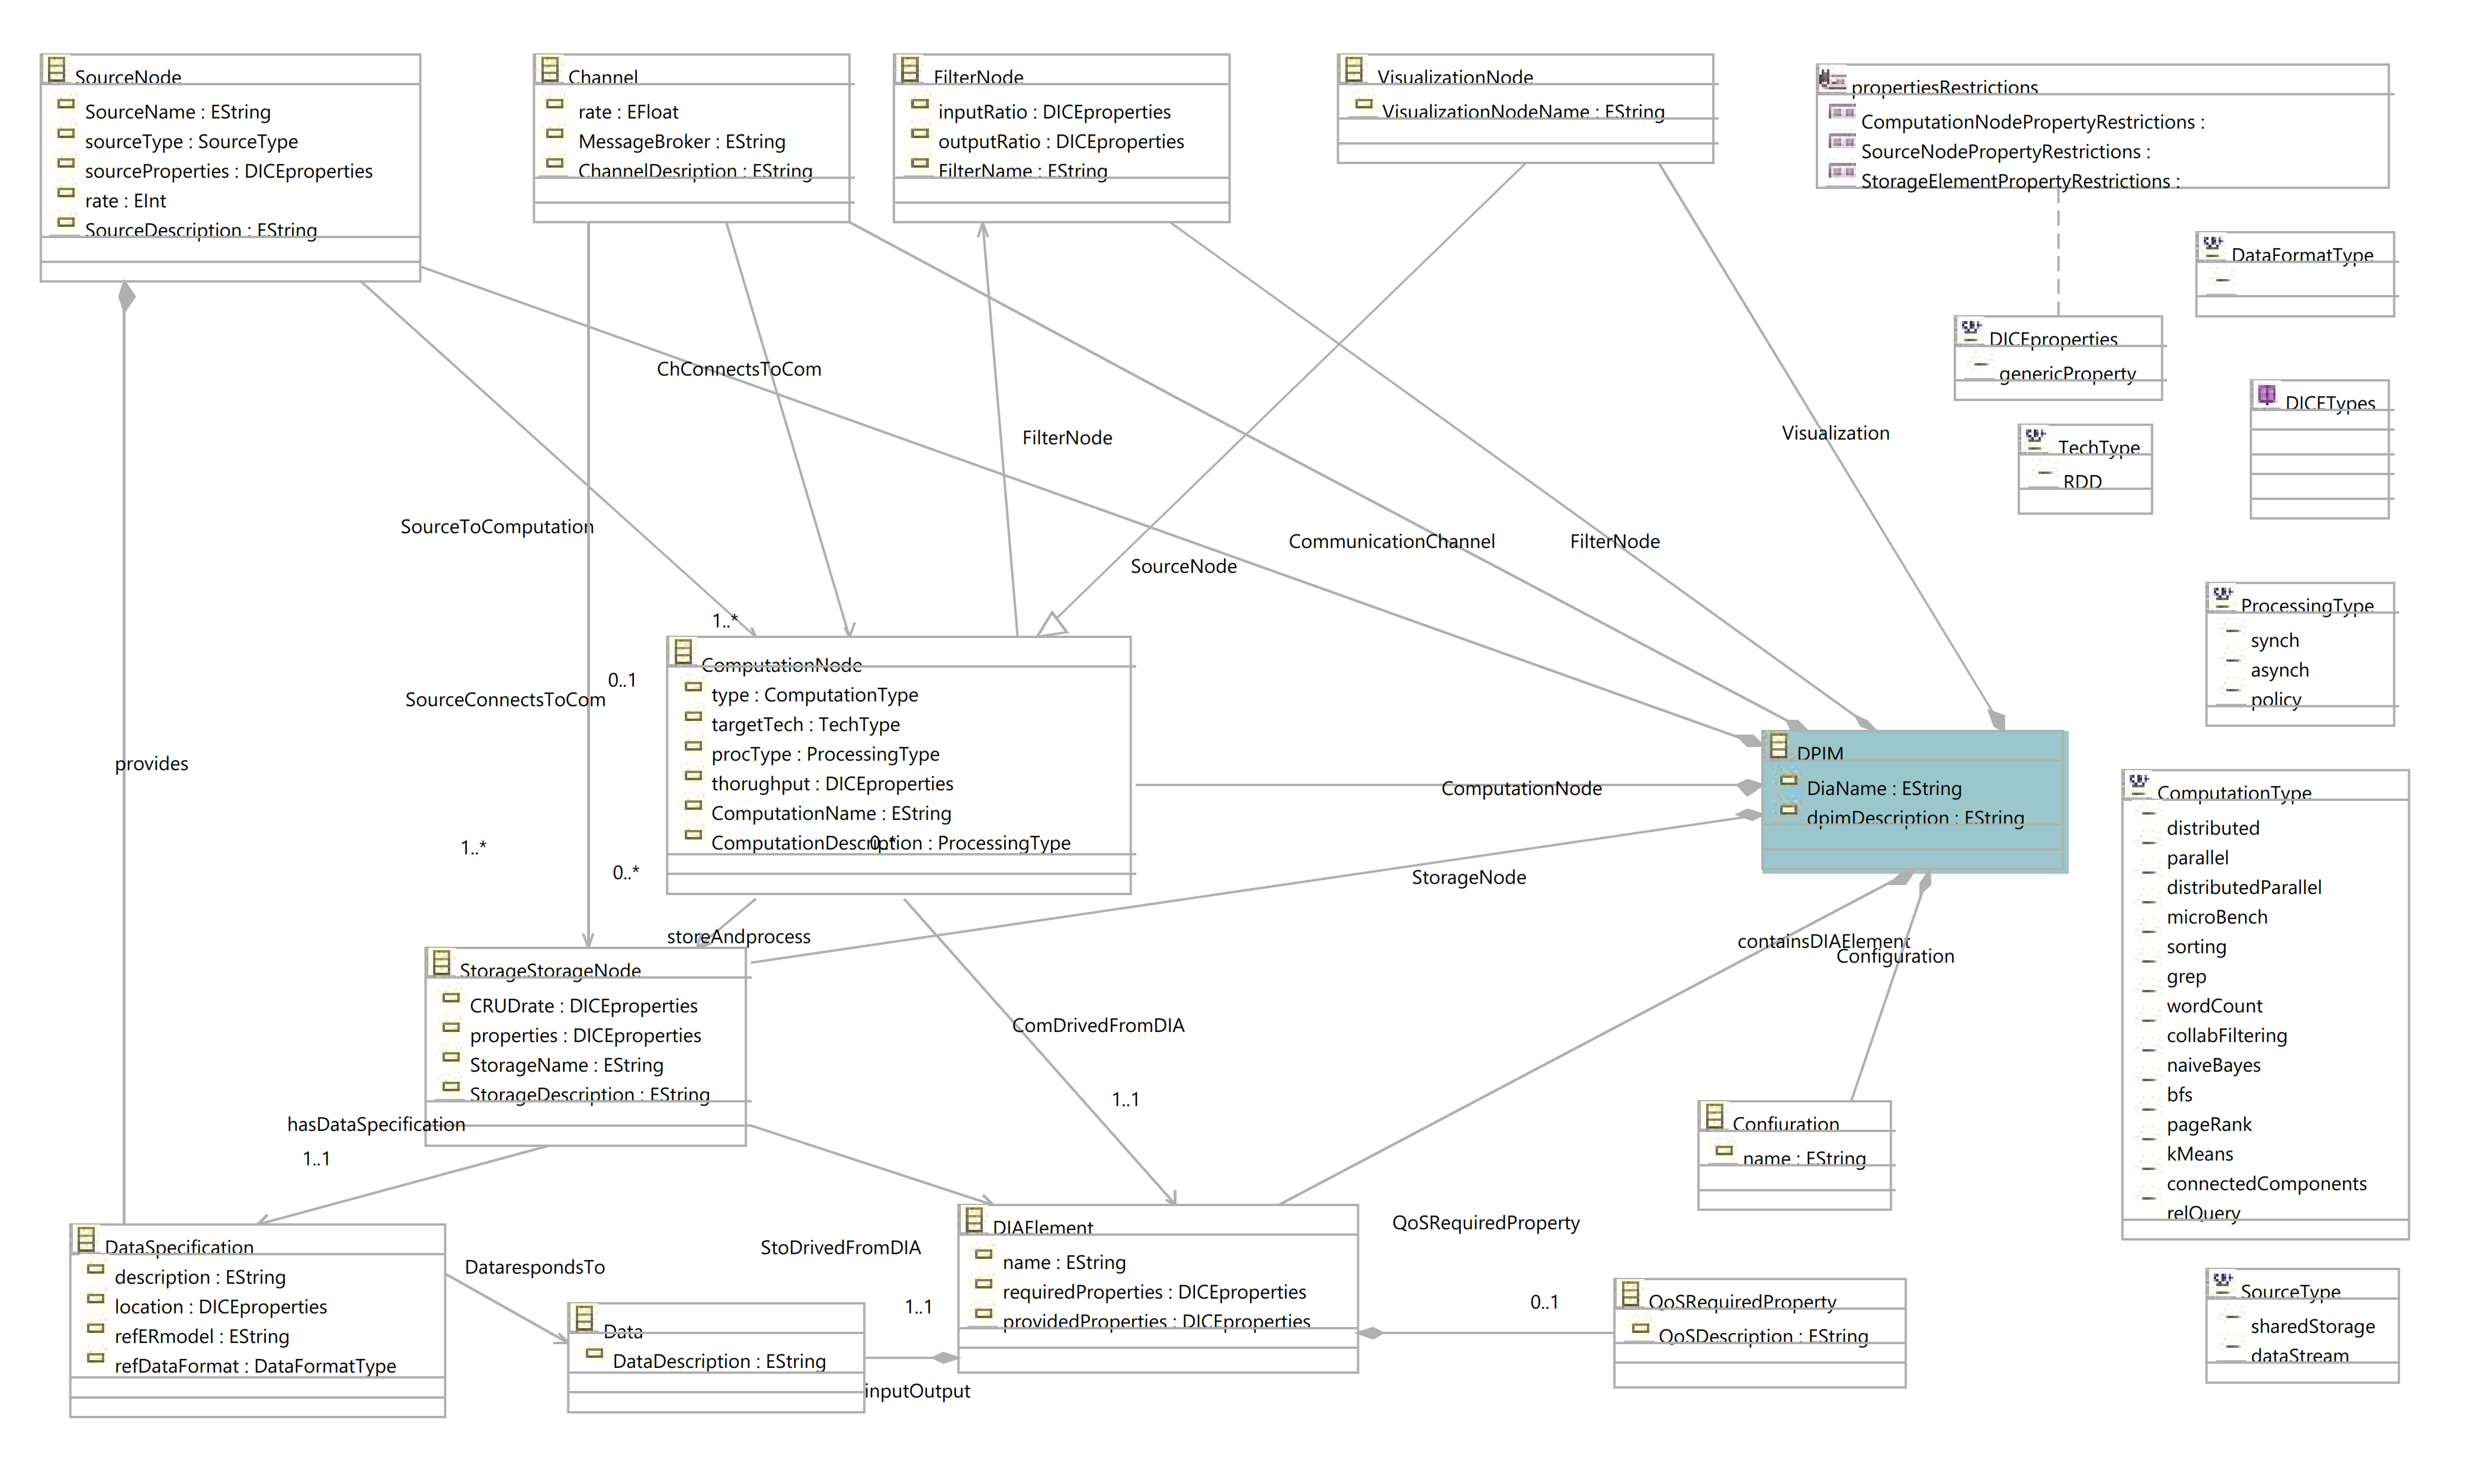
\includegraphics[width=0.8\textwidth]{Images/11.png}
    \caption{High-level Class Diagram}
    \label{fig:class-diagram}
\end{figure}

\subsection{Product Functions}

\subsection{User characteristics}

\subsection{Assumptions, dependencies and constraints}

\subsubsection{Domain Assumptions}
\begin{center}
    {\renewcommand{\arraystretch}{2}
    \begin{tabularx}{\textwidth}{p{2cm} X}
        \hline
        \textbf{ID} & \textbf{Description} \\ \hline
        D1 & Internship descriptions are comprehensive and reliable \\ \hline
        D2 & CVs accurately reflect students' skills and experiences \\ \hline
        D3 & Universities actively oversee internships and intervene when necessary \\ \hline
        D4 & Companies manage interview timelines and conduct them professionally \\ \hline
        D5 & Users provide meaningful feedback to improve the system \\ \hline
        D6 & Problems are reported in a timely manner by all parties \\ \hline
        D7 & The platform supports high user traffic without performance issues \\ \hline 
    \end{tabularx}}
\end{center}